\section{Auswertung}
\label{sec:evaluation}
In diesem Abschnitt wird die Lebensdauer komischer Myonen aus den Messdaten gewonnen.
Um dieses Ziel zu erreichen, ist es erforderlich die Messapparatur zu kalbibrieren.
Alle Fehler werden im Folgenden mit Hilfe
des \texttt{python}-Paktes \texttt{uncertainties} \cite{uncertain} berechnet, welches eine automatische
Gauß'sche Fehlerfortpflanzung bereitstellt.

\subsection{Kalibrierung der Messapparatur}
\label{subsec:calibration}
Die Daten über die Lebensdauer wird mit Hilfe eines Vielkanalanalysators (VKA) gewonnen. Der VKA teilt die gemessenen Lebensdauern in \num{512} Kanäle (Bins) eines Histogrammes ein. Dabei ist zu berücksichtigen, das der Zusammenghang zwischen gemessener Lebensdauer und Kanal linear zusammenhängt. Somit ist es Sinnvoll dieses Zusammenhang über eine lineare Funktion
\begin{equation}
f(c) = Ac + B
\end{equation}
anzunehmen.

\begin{figure}[h!]
	\centering
	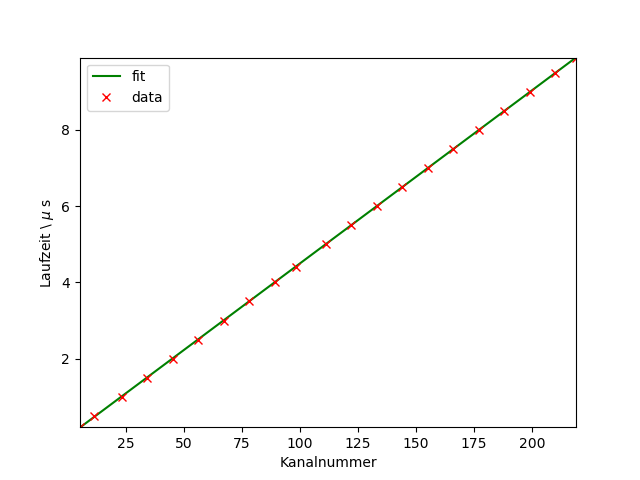
\includegraphics[width=\textwidth]{img/calib.png}
	\caption{Lineare Ausgleichsrechnung zur Bestimmung der proportionalität zwischen Kanälen und Zeit}
	\label{abb:cal}
\end{figure}

\noindent Die Ausgleichsrechnung in \autoref{abb:cal} an die Werte in \autoref{tab:calib} liefert somit
\begin{equation}
	t(c) = (0.0454 \pm 0.00003)\frac{\si{\micro\second}}{\text{Kanal}} - (0.035 \pm 0.004) \si{\micro\second}
\end{equation}
Im der weiteren Auswertung ist lediglich der Parameter $A$ von Interesse, da dieser die Wartezeit pro Kanal beschreibt und somit den Zusammenhang zwischen VKA Kanal und Wartezeit liefert. Sollten mehrere Kanäle im VKA gefüllt worden sein, wurde über die betroffenen Kanalnummern gemittelt.

\subsection{Zeitauflösung der Messapparatur}
\label{subsec:timeresolution}
Um verschiedene Signallaufzeiten zwischen den SEV's und der Koinzidenz ausgleichen zu können, werden Verzögerungsleitungen benutzt, um weitere Verzögerungen in das System einbringen zu können. Durch Messung der Myonen-Zählrate unter Variation der Verzögerungszeiten lässt sich die Auflösungszeit $\Delta t_\text{K}$ der Koinzidenzschaltung als Breite der Verteilung der Zählrate in Abhängigkeit von der Verzögerung bestimmen. Die Verteilung hat im Allgemeinen abfallende Flanken zu größeren Verzögerungszeiten und erreicht dazwischen einen Plateauwert.
\begin{figure}
	\centering
	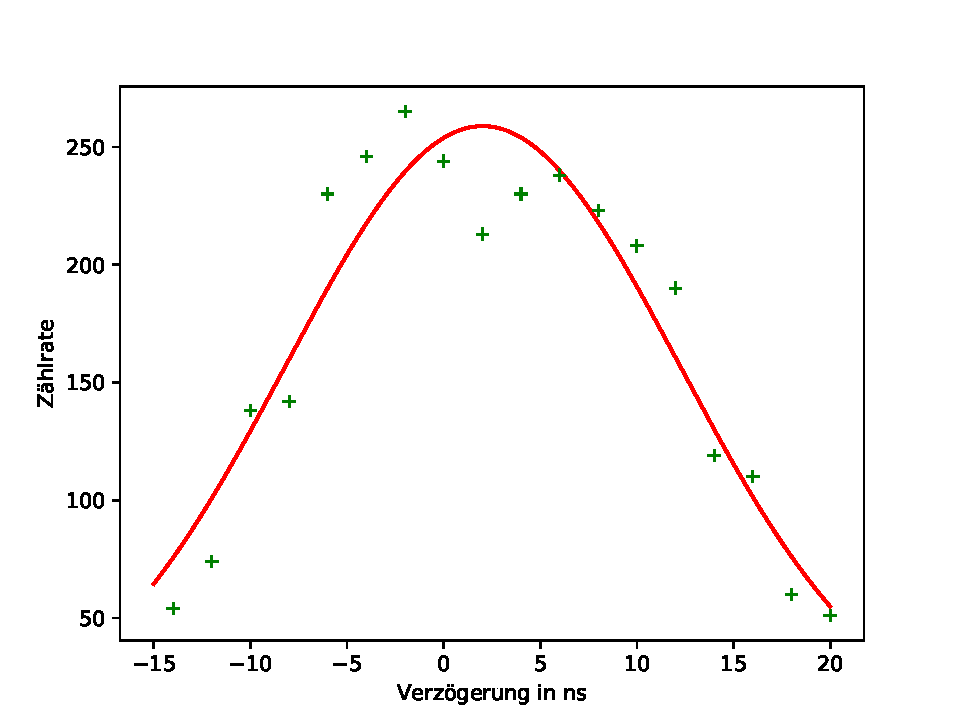
\includegraphics[width=\textwidth]{img/res.pdf}
	\caption{Myon-Zählraten unter Variation der Verzögerungszeit}
	\label{abb:res}
\end{figure}
Statt einer Trapezfunktion wurde aus Gründen der Einfachheit eine Gaußglocke der Form
\begin{equation}
	\text{Zählrate} = A \cdot \exp\left\{\frac{-(x - \mu)^2}{2 \sigma^2}\right\}
\end{equation}
an die Messwerte gefittet. Die Fitparameter sind $A = 258.8 \pm 10.5$, $\mu = 2.0 \pm 0.5$ und $\sigma = 10.21 \pm 0.56$. Aus \autoref{abb:res} ergibt sich aus der Halbwertsbreite eine Zeitauflösung von $\Delta t_k = \SI{24.03}{\nano\second}$.

\subsection{Untergrundrate}
\label{subsec:underground}

Um die Untergrundrate $N_\text{B}$ abschätzen zu können, wird die Wahrscheinlichkeit betrachtet, mit der ein Myon im Tank bei gestarteter Messung in einem Zeitintervall von $T_\text{S} = \SI{10}{\micro\second}$ ein Stopp-Signal erzeugt. Unter der Annahme dass das Auftreten von Myonen normalverteilt ist, lässt sich die Wahrscheinlichkeit $p_i$ einer Messung von $i$ Myonen durch eine Poissonverteilung abschätzen:

\begin{equation}
p_i = \frac{\lambda^i}{i!}\mathrm{e}^{-\lambda}\,,
\end{equation}

\noindent wobei der Erwarungswert der Messung eines Myons mit $\lambda$ bezeichnet wird. Dieser Erwarungswert wird mit der Myonenzählrate identifiziert. Somit liefert die Poissonverteilung die Wahrscheinlichkeit
für die Messung eines Myons.

\noindent Zur Berechnung der Untergrundrate ist es notwendig, die durchschnittliche Anzahl an Myonen zu bestimmen, die in einer Sekunde den Tank passieren.
Die durchgeführte Messung liefert $N_{\text{Start}} = 1426728$ und $t_{\text{Messung}} = \SI{513670}{\second}$.

\begin{equation}
f = \frac{N_{\text{Start}}}{t_{\text{Messung}}} = 2,28 \, \frac{\text{Myonen}}{\text{s}}
\end{equation}

\noindent Die Wahrscheinlichkeit, dass genau ein weiteres Myon innerhalb der Suchzeit den Tank durchquert, berechnet sich gemäß

\begin{equation}
P = \frac{(T_s \cdot f)^k}{k!} \exp{(f \cdot T_s)} = 2.28 \cdot 10^{-5},
\end{equation}
wobei k = 1 gilt. Somit ergeben sich bezogen auf die Startimpulse

\begin{equation}
N_{Err} = 32.53
\end{equation}

\noindent Fehlmessungen. Werden jetzt noch die einzelnen Kanäle berücksichtigt ergibt sich folgende Untergrundrate pro Kanal:

\begin{equation}
U_{\text{B}} = 0,07 \, \frac{\text{Ereignisse}}{\text{Kanal}}\,.
\end{equation}

\subsection{Bestimmung der Lebensdauer}
\label{subsec:lifetime}
Zur bestimmung der Individuallebensdauer der Myonen werden in \autoref{abb:fit} die Daten an eine Exponentialfunktion gemäß
\begin{equation}
f(t) = N_0 \cdot \exp{( -\lambda t)} + U_{\text{B}}
\end{equation}
gefittet, wobei $U_{\text{B}}$ die Untergrundrate und $\lambda$ die Zerfallskonstante ist.
\begin{figure}[h!]
	\centering
	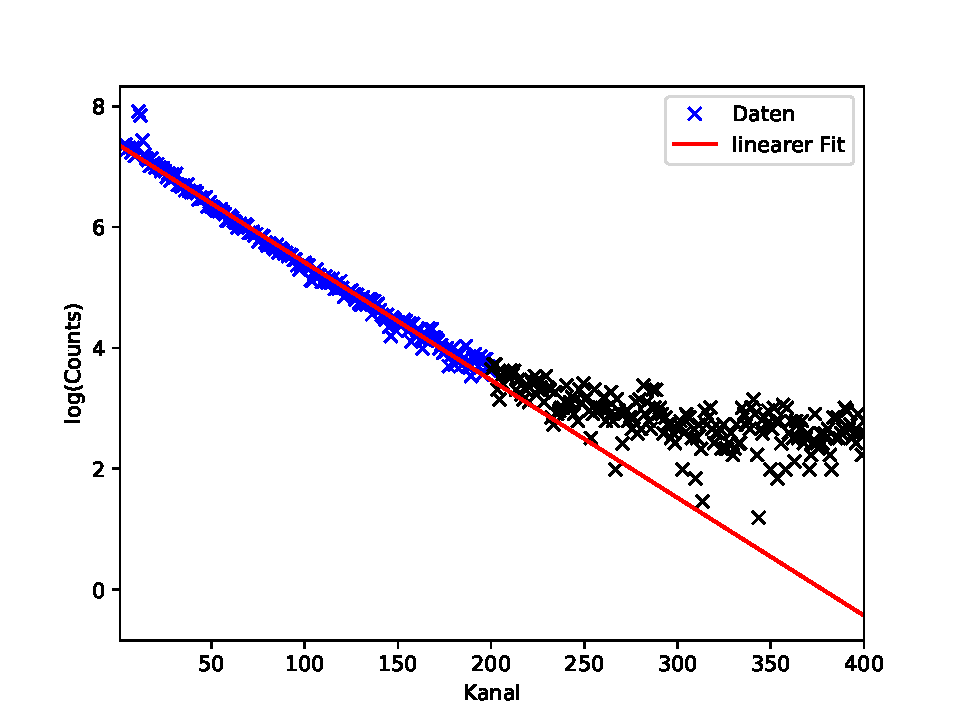
\includegraphics[width=\textwidth]{img/myons.pdf}
	\caption{Exponentielle Ausgleichsrechnung zur Bestimmung der Zerfallskonstante}
	\label{abb:fit}
\end{figure}
Die Ausgleichsrechnung liefert die Parameter $N_0 = 1691.34 \pm 31.88$, $\lambda = 0.0208 \pm 0.0006$\,1/Kanal und $U_\text{B} = 10.05 \pm 6.32$. Hierbei ist zu beachten, dass die Zerfallskonstante in Abhängigkeit des Kanals des VKA bestimmt wurde. Mithilfe der Kalibration durch die lineare Ausgleichsrechnung in \autoref{subsec:calibration} wird der Kanal in eine Zeit umgerechnet. Mit dem Umrechnungsfaktor $F = (0.0454 \pm 0.00003) \,$ \si{\micro\second}/Kanal ist die Lebensdauer $\tau = F / \lambda$, also
\begin{equation}
\tau = \SI[separate-uncertainty=true]{2.1789(14)}{\micro\second} \, .
\end{equation}
